\documentclass{article}
\usepackage[top=20mm, left=20mm, right=20mm]{geometry}
\usepackage[dvipsnames]{xcolor}
\usepackage{graphicx}
\usepackage{enumerate}
\usepackage{amsmath}
\usepackage{amsfonts}
\usepackage{amsthm}
\usepackage{multicol}
\usepackage{fontspec}
\usepackage{float, graphicx}
\usepackage{cancel}
\usepackage{framed}
\usepackage{tikz}
\usepackage{tkz-euclide}
\usepackage{pgfplots}
\usepackage{amssymb}
\usepackage{gensymb}
\usepackage{xfrac}
\pgfplotsset{compat=1.8}
\usetikzlibrary{automata, positioning, arrows, calc, angles, quotes}
\tikzset{style={font=\scriptsize}}
\usetkzobj{all}
\newcommand{\defLang}[1]{L = \big\{ #1 \big\}}
\newcommand{\derives}{\rightarrow}
\newcommand{\blank}{\textbf{\textvisiblespace}}
\newcommand{\proofend}{\quad\blacksquare}
\newcommand{\question}[1]{\section*{Question #1}\vspace{.5cm}}
\newcommand{\separator}{\vspace{.3cm}\begin{center}\noindent\rule{15cm}{0.4pt}\end{center}\vspace{.3cm}}
\newcommand{\twoColumns}[4]{
    \begin{minipage}{#1\linewidth}#3\end{minipage}
    \begin{minipage}{#2\linewidth}#4\end{minipage}
}
\newcommand{\norm}[1]{\vert\vert#1\vert\vert}
\newcommand{\mappingreducible}{\leq_m}
\newcommand{\TMdefinition}[2]{\begin{framed}#1: #2\end{framed}}
\newcommand{\complexity}[1]{O\big(#1\big)}
\newcommand{\header}[1]{\underline{#1}\\}

\begin{titlepage}
    \title{\textbf{Computer Graphics - Ex. 4}}
    \author{Niv Shani, ID: 311361661}
    \date{}
\end{titlepage}

\begin{document}
    \maketitle
    \question{1}
    \begin{enumerate}
        \item \textsl{Rotate by $60\degree$ counter-clockwise around the z-axis, translate the origin to $(0,3,0)$ and scale uniformly by factor $2$.}\\\\
        \boxed{Similarity} transformation, given by:
        $$
            \underset{\textsl{uniform scaling}}{\begin{pmatrix}2&0&0&0\\0&2&0&0\\0&0&2&0\\0&0&0&1\end{pmatrix}}
            \cdot \underset{\textsl{translation}}{\begin{pmatrix}1&0&0&0\\0&1&0&3\\0&0&1&0\\0&0&0&1\end{pmatrix}}
            \cdot \underset{\textsl{rotation around z-axis}}{\begin{pmatrix}cos{60}&-sin60&0&0\\sin60&cos60&0&0\\0&0&1&0\\0&0&0&1\end{pmatrix}} = \begin{pmatrix}2cos60&-2sin60&0&0\\2sin60&2cos60&0&6\\0&0&2&0\\0&0&0&1\end{pmatrix}\proofend
        $$
        \item \textsl{Reflect about $xy$ plane, then scale by $0.5$ in $\big(\frac{1}{\sqrt{2}}, \frac{1}{\sqrt{2}}, 0\big)$-direction.}\\\\
        \boxed{Linear} transformation.\\\\
        To scale in the given direction we need to align it with one of the main axes. To do so, we need to first construct an orthonormal basis, containing the scale direction $\vec{u} = \big(\frac{1}{\sqrt{2}}, \frac{1}{\sqrt{2}}, 0\big)$. We can see that one orthogonal vector can be $\vec{v} = \big(\frac{1}{\sqrt{2}}, -\frac{1}{\sqrt{2}}, 0\big)$, and thus a third orthogonal vector can be $w=(0,0,1)$. Indeed we have:
        \begin{align*}
            &\vec{u}\cdot\vec{v} = \frac{1}{\sqrt{2}}\cdot\frac{1}{\sqrt{2}}-\frac{1}{\sqrt{2}}\cdot\frac{1}{\sqrt{2}}+0\cdot 0 = 0\qquad\qquad
            \vec{u}\cdot\vec{w} = \frac{1}{\sqrt{2}}\cdot0+\frac{1}{\sqrt{2}}\cdot0+0\cdot1 = 0\\
            &\vec{v}\cdot\vec{w} = \frac{1}{\sqrt{2}}\cdot0-\frac{1}{\sqrt{2}}\cdot0+0\cdot1 = 0\qquad\qquad\qquad
            \norm{u} = \norm{v} = \norm{w} = 1
        \end{align*}
        Therefore $(u,v,w)$ is a orthonormal basis. Denote the change of basis matrix from $(u,v,w)$ to $(x,y,z)$ as $P$. Thus the opposite direction matrix defined by (using homogeneous coordinates):
        $$
            P^{-1} = P^T = \begin{pmatrix}
                \sfrac{1}{\sqrt{2}}&\sfrac{1}{\sqrt{2}}&0&0\\
                \sfrac{1}{\sqrt{2}}&-\sfrac{1}{\sqrt{2}}&0&0\\
                0&0&1&0\\
                0&0&0&1
            \end{pmatrix}
        $$
        This rotation matrix aligns $\vec{u}$ - the given scaling direction, with the $x$-axis. Therefore we only need to scale in the $x$-axis direction, and then apply the reverse operations. Therefore the overall transformation is given by:
        $$
            \underset{\textsl{reverse alignment ($P=P^T$)}}{\begin{pmatrix}
                \sfrac{1}{\sqrt{2}}&\sfrac{1}{\sqrt{2}}&0&0\\
                \sfrac{1}{\sqrt{2}}&-\sfrac{1}{\sqrt{2}}&0&0\\
                0&0&1&0\\
                0&0&0&1
            \end{pmatrix}}
            \cdot
            \underset{\textsl{scale about the $x$-axis}}{\begin{pmatrix}
                0.5&0&0&0\\
                0&1&0&0\\
                0&0&1&0\\
                0&0&0&1
            \end{pmatrix}}
            \cdot
            \underset{\textsl{align $u$ to $x$-axis}}{\begin{pmatrix}
                \sfrac{1}{\sqrt{2}}&\sfrac{1}{\sqrt{2}}&0&0\\
                \sfrac{1}{\sqrt{2}}&-\sfrac{1}{\sqrt{2}}&0&0\\
                0&0&1&0\\
                0&0&0&1
            \end{pmatrix}}
            \cdot
            \underset{\textsl{xy-plane reflection}}{\begin{pmatrix}1&0&0&0\\0&1&0&0\\0&0&-1&0\\0&0&0&1\end{pmatrix}}\proofend
        $$
        \newpage
        \item \textsl{Project (perspective) at the direction of the origin on the view plane $z=-2$, then reflect about the $x=-y$ line.}\\\\
        \boxed{Projective} transformation, given by:
        $$
            \underset{\textsl{reflection}}{
                \begin{pmatrix}
                    0&-1&0&0\\
                    -1&0&0&0\\
                    0&0&1&0\\
                    0&0&0&1
                \end{pmatrix}
            }
            \cdot
            \underset{\textsl{perpective projection}}{
                \begin{pmatrix}
                    1&0&0&0\\
                    0&1&0&0\\
                    0&0&0&0\\
                    0&0&-\sfrac{1}{2}&1
                \end{pmatrix}
            }
            =
            \begin{pmatrix}
                0&-1&0&0\\
                -1&0&0&0\\
                0&0&0&0\\
                0&0&-\sfrac{1}{2}&1
            \end{pmatrix}\proofend
        $$
    \end{enumerate}
    \vspace{1cm}
    \question{2}
    \begin{enumerate}
        \item \textsl{
            Prove that 2D reflection about the line $y=xtan\theta$, where $\theta$ is the angle between the line the $x$ axis is given by:
            $$\begin{pmatrix}cos2\theta&sin2\theta\\sin2\theta&-cos2\theta\end{pmatrix}$$
            \\\\
            \noindent
            Notice that the operations we need to use are rotation and scaling (reflection), meaning the transformation is linear. Therefore we won't need to use homogeneous coordinates.
        }\\\\
        First, we rotate the line $y=xtan\theta$ to make it coincident with the $x$ axis. We do that by rotating it by $\theta$ degrees \textbf{clockwise} - so we'll use the inverse rotation matrix:
        \begin{equation}
            \begin{pmatrix}
                cos(-\theta)&-sin(-\theta)\\sin(-\theta)&cos(-\theta)
            \end{pmatrix} \quad\Longrightarrow\quad
            \begin{pmatrix}
                cos\theta&sin\theta\\-sin\theta&cos\theta
            \end{pmatrix}
        \end{equation}
        We'll now use a reflection around the $x$ axis:
        \begin{equation}
            \begin{pmatrix}
                1&0\\0&-1
            \end{pmatrix}
        \end{equation}
        And now rotate $\theta$ degrees back (\textbf{counter-clockwise}):
        \begin{equation}
            \begin{pmatrix}
                cos\theta&-sin\theta\\
                sin\theta&cos\theta
            \end{pmatrix}
        \end{equation}
        We'll now multiply (3), (2) and (1) to get the matrix reprsenting this affine transformation:
        \begin{align*}
            &\begin{pmatrix}
                cos\theta&-sin\theta\\
                sin\theta&cos\theta
            \end{pmatrix}
            \cdot
            \begin{pmatrix}
                1&0\\0&-1
            \end{pmatrix}
            \cdot
            \begin{pmatrix}
                cos\theta&sin\theta\\-sin\theta&cos\theta
            \end{pmatrix}\\\\
            &= \begin{pmatrix}
                cos\theta&sin\theta\\
                sin\theta&-cos\theta
            \end{pmatrix}
            \cdot
            \begin{pmatrix}
                cos\theta&sin\theta\\-sin\theta&cos\theta
            \end{pmatrix}\\\\
            &= \begin{pmatrix}
                cos^2\theta-sin^2\theta&2sin\theta cos\theta\\
                2sin\theta cos\theta&sin^2\theta -cos^2\theta
            \end{pmatrix}\\\\
            &\stackrel{=}{\textsl{\scriptsize identities}}
            \begin{pmatrix}
                cos2\theta&sin2\theta\\
                sin2\theta&-cos2\theta
            \end{pmatrix}\proofend
        \end{align*}

    \item \textsl{
        Show that a 2D rotation matrix, can be factorized into three shear matrices:
        $$
            \begin{pmatrix}
                cos\theta&-sin\theta\\cos\theta&sin\theta
            \end{pmatrix} =
            \begin{pmatrix}1&s_1\\0&1\end{pmatrix}\cdot
            \begin{pmatrix}1&0\\s_2&1\end{pmatrix}\cdot
            \begin{pmatrix}1&s_3\\0&1\end{pmatrix}
        $$
    }
    \\\\
    \noindent
    Set $s_1 = s_3 = -tan\frac{\theta}{2},\ s_3 = sin\theta$.\\
    A rotation is a linear transformation, thus we can multiply the matrices:
    $$
        \begin{pmatrix}1&-tan\frac{\theta}{2}\\0&1\end{pmatrix}\cdot
        \begin{pmatrix}1&0\\sin\theta&1\end{pmatrix}\cdot
        \begin{pmatrix}1&-tan\frac{\theta}{2}\\0&1\end{pmatrix} =
        \begin{pmatrix}
            1-sin\theta tan\frac{\theta}{2}& -tan\frac{\theta}{2}(1-sin\theta tan\frac{\theta}{2}) -tan\frac{\theta}{2}\\
            sin\theta& 1-sin\theta tan\frac{\theta}{2}
        \end{pmatrix}
    $$
    Using the following identities:
    $$tan\frac{\alpha}{2} = \dfrac{1-cos\alpha}{sin\alpha}\qquad\qquad sin^2\alpha + cos^2\alpha = 1$$
    We have:
    $$
        \begin{pmatrix}
            1-(1-cos\theta)&-\frac{1-cos\theta}{sin\theta}(1-(1-cos\theta)) -\frac{1-cos\theta}{sin\theta}\\
            sin\theta& 1-(1-cos\theta)
        \end{pmatrix} =
        \begin{pmatrix}
            cos\theta&-\frac{1-cos\theta}{sin\theta}\big[1+cos\theta\big]\\
            sin\theta&cos\theta
        \end{pmatrix}
    $$
    $$
        = \begin{pmatrix}
            cos\theta&-\frac{1-cos^2\theta}{sin\theta}\\
            sin\theta&cos\theta
        \end{pmatrix}
        = \begin{pmatrix}
            cos\theta&-sin\theta\\
            sin\theta&cos\theta
        \end{pmatrix}
    $$
    \\\\
    \noindent
    For $\theta = 90\degree$, we have $s_1 = s_3 = -tan(45\degree) = -1,\ s_2 = sin(90\degree) = 1$:\\
    \begin{figure}[!htb]
        \begin{minipage}{0.33\textwidth}
            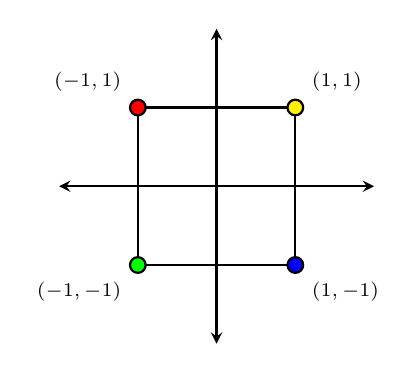
\begin{tikzpicture}[>=stealth,dot/.style={circle,draw=black,inner
                sep=2pt},black,thick,every label/.style={black}]
                \draw[<->] (-2,0) -- (2,0);
                \draw[<->] (0,-2) -- (0,2);
                \draw (-1,1) node[dot,fill=red,label=above left:{$(-1, 1)$}] {}
                -- (-1,-1) node[dot,fill=green,label=below left:{$(-1,-1)$}] {}
                -- (1,-1) node[dot,fill=blue,label=below right:{$(1,-1)$}] {}
                -- (1,1) node[dot,fill=yellow,label=above right:{$(1,1)$}] {} -- cycle;
            \end{tikzpicture}\\
            \centering \textsl{\scriptsize initial square}
        \end{minipage}
        \begin{minipage}{0.33\textwidth}
            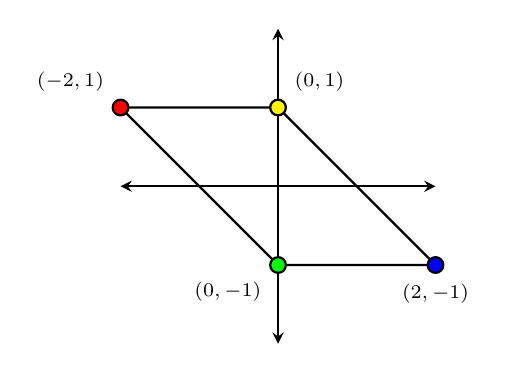
\begin{tikzpicture}[>=stealth,dot/.style={circle,draw=black,inner
                sep=2pt},black,thick,every label/.style={black}]
                \draw[<->] (-2,0) -- (2,0);
                \draw[<->] (0,-2) -- (0,2);
                \draw (-2,1) node[dot,fill=red,label=above left:{$(-2, 1)$}] {}
                -- (0,-1) node[dot,fill=green,label=below left:{$(0,-1)$}] {}
                -- (2,-1) node[dot,fill=blue,label=below:{$(2,-1)$}] {}
                -- (0,1) node[dot,fill=yellow,label=above right:{$(0,1)$}] {} -- cycle;
            \end{tikzpicture}\\
            \centering \textsl{\scriptsize applying rightmost matrix}
        \end{minipage}
        \begin{minipage}{0.33\textwidth}
            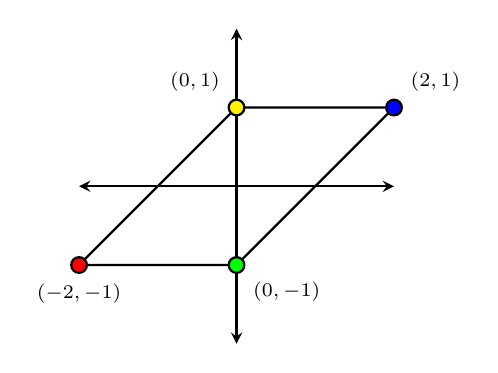
\begin{tikzpicture}[>=stealth,dot/.style={circle,fill=black!50,draw=black,inner
                sep=2pt},black,thick,every label/.style={black}]
                \draw[<->] (-2,0) -- (2,0);
                \draw[<->] (0,-2) -- (0,2);
                \draw (-2,-1) node[dot,fill=red,label=below:{$(-2, -1)$}] {}
                -- (0,-1) node[dot,fill=green,label=below right:{$(0,-1)$}] {}
                -- (2,1) node[dot,fill=blue,label=above right:{$(2,1)$}] {}
                -- (0,1) node[dot,fill=yellow,label=above left:{$(0,1)$}] {} -- cycle;
            \end{tikzpicture}\\
            \centering \textsl{\scriptsize applying center matrix}
        \end{minipage}
    \end{figure}
    \\
    \noindent and finally applying the leftmost matrix, to complete a $90\degree$ rotation (counter-clockwise):
    \begin{figure}[h!]
        \centering
        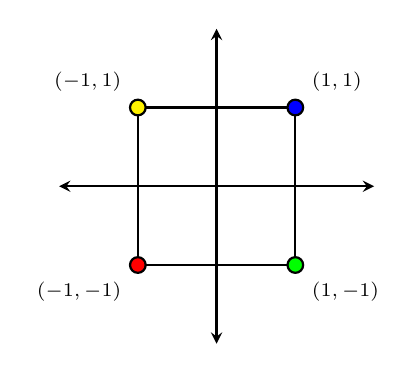
\begin{tikzpicture}[>=stealth,dot/.style={circle,fill=black!50,draw=black,inner
            sep=2pt},black,thick,every label/.style={black}]
            \draw[<->] (-2,0) -- (2,0);
            \draw[<->] (0,-2) -- (0,2);
            \draw (-1,-1) node[dot,fill=red,label=below left:{$(-1, -1)$}] {}
            -- (1,-1) node[dot,fill=green,label=below right:{$(1,-1)$}] {}
            -- (1,1) node[dot,fill=blue,label=above right:{$(1,1)$}] {}
            -- (-1,1) node[dot,fill=yellow,label=above left:{$(-1,1)$}] {} -- cycle;
        \end{tikzpicture}
    \end{figure}\\
    $\proofend$
    \item \textsl{
        Find the reflection matrix about the plane:
    $$(p-q)\cdot n = 0\qquad s.t\qquad q=(q_x,q_y,q_z)\in\mathbb{R}^3\textsl{ a point on the plane},\quad \vec{n}=(n_x,n_y,n_z) \textsl{ is the plane normal}$$
    }
    \\\\
    \noindent Denote:
    $$\norm{n} = \sqrt{n_x^2+n_y^2+n_z^2}$$

    Let $p=(x,y,z)$ a general point. We'll find it's reflection about the given plane, and consruct the transformation matrix accordingly.\\\\
    Denote the vector from $q$ to $p$:

    $$\vec{v} = p - q = (x-q_x, y-q_y, z-q_z)$$

    Therefore, the signed distance of $p$ from the plane, is given by:

    $$d = \frac{\vec{v}\cdot \vec{n}}{\norm{n}} = \frac{(x-q_x)n_x+(y-q_y)n_y+(z-q_z)n_z}{\sqrt{n_x^2+n_y^2+n_z^2}}$$

    Notice that for any plane, the reflection of any point with a signed distance $d$ from it is given by "moving" the point $2d$ units in the negative direction of the normal - therefore, the reflected point $\hat{p}$ is given by:

    $$\hat{p} = p - 2dn = p-\frac{2\vec{v}\cdot\vec{n}}{\norm{n}^2}\cdot n = (x,y,z) - 2\cdot\frac{(x-q_x)n_x+(y-q_y)n_y+(z-q_z)n_z}{n_x^2+n_y^2+n_z^2}$$

    Looking at each component separately, we can derive the transformation in each component:

    $$
        T_x = \left(1-\frac{2n_x}{n_x^2+n_y^2+n_z^2}\right)x + \frac{n_xq_x}{n_x^2+n_y^2+n_z^2}
    $$
    $$
        T_y = \left(1-\frac{2n_y}{n_x^2+n_y^2+n_z^2}\right)y + \frac{n_yq_y}{n_x^2+n_y^2+n_z^2}
    $$
    $$
        T_z = \left(1-\frac{2n_z}{n_x^2+n_y^2+n_z^2}\right)z + \frac{n_zq_z}{n_x^2+n_y^2+n_z^2}
    $$

    We can see that the transformation in each component is a combination of scaling and translation. Thus the reflection matrix is given by:

    $$
        \begingroup
            \renewcommand*{\arraystretch}{2.2}
            T = \begin{pmatrix}
                1-\dfrac{2n_x}{n_x^2+n_y^2+n_z^2}&0&0&\dfrac{n_xq_x}{n_x^2+n_y^2+n_z^2}\\
                0&1-\dfrac{2n_y}{n_x^2+n_y^2+n_z^2}&0&\dfrac{n_yq_y}{n_x^2+n_y^2+n_z^2}\\
                0&0&1-\dfrac{2n_z}{n_x^2+n_y^2+n_z^2}&\dfrac{n_zq_z}{n_x^2+n_y^2+n_z^2}\\
                0&0&0&1
            \end{pmatrix}
        \endgroup\proofend
    $$
    \end{enumerate}

    \newpage
    \question{3}
    \textsl{
    Given a cube with vertices at
    $(0,0,0),\ (0,0,1),\ (1,0,0),\ (0,1,0),\ (1,1,0),\ (1,0,1),\ (0,1,1),\ (1,1,1)$.\\
    For each of the following diagrams, find the parallel projection matrix that will project the cube upon the given shape, in the $xy$-plane (in which $z=0$).
    }
    \vspace{.5cm}
    \begin{enumerate}
        \item \twoColumns{0.25}{0.75}{
            \centering
            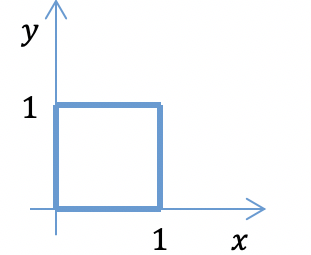
\includegraphics[width=4cm]{q3_1.png}
        }{
            The given projection is a simple parallel projection to the $z=0$ plane, given by the matrix:
            $$
                P_1 = \begin{pmatrix}
                    1&0&0&0\\
                    0&1&0&0\\
                    0&0&0&0\\
                    0&0&0&1
                \end{pmatrix}\proofend
            $$
        }
        \separator
        \item \twoColumns{0.25}{0.75}{
            \centering
            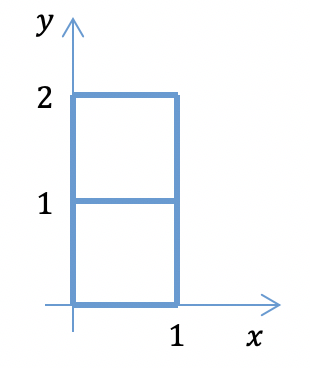
\includegraphics[width=4cm]{q3_2.png}
        }{
            The given projection is an Oblique projection. We can see that the projected point of the point $(1,1,1)$, for example, is $p = (1,2,0)$. Plugging $z=1$ we have:
            $$
                x_p = 1 = 1 + \dfrac{1}{tan\alpha}\cdot cos\phi\qquad\qquad
                y_p = 2 = 1 + \dfrac{1}{tan\alpha}\cdot sin\phi
            $$
            therefore,
            $$
                \dfrac{cos\phi}{tan\alpha} = 0\qquad\qquad\qquad
                \dfrac{sin\phi}{tan\alpha} = 1
            $$
            Thus the projection is defined by the projection matrix:
            $$
                P_2 = \begin{pmatrix}
                    1&0&\frac{cos\phi}{tan\alpha}&0\\
                    0&1&\frac{sin\phi}{tan\alpha}&0\\
                    0&0&0&0\\
                    0&0&0&1
                \end{pmatrix} =
                \begin{pmatrix}
                    1&0&0&0\\
                    0&1&1&0\\
                    0&0&0&0\\
                    0&0&0&1
                \end{pmatrix}\proofend
            $$
        }
        \separator
        \item \twoColumns{0.25}{0.75}{
            \centering
            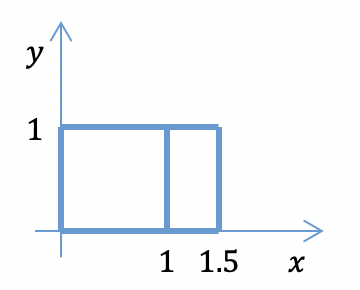
\includegraphics[width=4cm]{q3_3.png}
        }{
            Following the same claims from secion (2), looking at $(1,1,1)$ we can see it's projection is $p = (1.5, 1, 0)$, which implies:
            $$
                x_p = 1.5 = 1 + \dfrac{1}{tan\alpha}\cdot cos\phi\qquad\qquad
                y_p = 1 = 1 + \dfrac{1}{tan\alpha}\cdot sin\phi
            $$
            therefore,
            $$
                \dfrac{cos\phi}{tan\alpha} = \dfrac{1}{2}\qquad\qquad\qquad
                \dfrac{sin\phi}{tan\alpha} = 0
            $$
            Thus the projection is defined by the projection matrix:
            $$
                P_3 = \begin{pmatrix}
                    1&0&\sfrac{1}{2}&0\\
                    0&1&0&0\\
                    0&0&0&0\\
                    0&0&0&1
                \end{pmatrix}\proofend
            $$
        }
        \newpage
        \item \twoColumns{0.25}{0.75}{
            \centering
            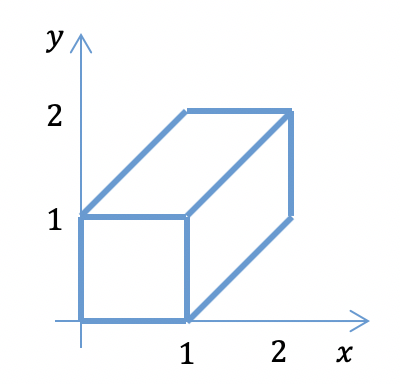
\includegraphics[width=4cm]{q3_4.png}
        }{
            For the point $(1,1,1)$ we have the projection $p=(2,2,0)$. Thus again:
            $$
                x_p = 2 = 1 + \dfrac{1}{tan\alpha}\cdot cos\phi\qquad\qquad
                y_p = 2 = 1 + \dfrac{1}{tan\alpha}\cdot sin\phi
            $$
            therefore,
            $$
                \dfrac{cos\phi}{tan\alpha} = \dfrac{sin\phi}{tan\alpha} = 1
            $$
            hence the projection matrix is:
            $$
                P_4 = \begin{pmatrix}
                    1&0&1&0\\
                    0&1&1&0\\
                    0&0&0&0\\
                    0&0&0&1
                \end{pmatrix}\proofend
            $$
        }
        \separator
        \item \twoColumns{0.25}{0.75}{
            \centering
            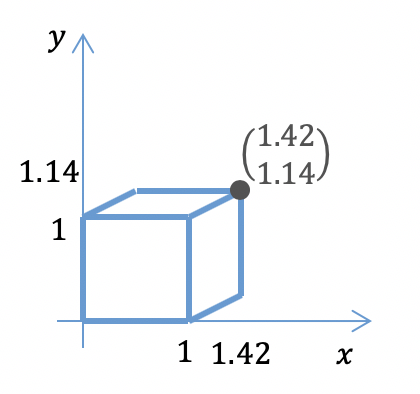
\includegraphics[width=4cm]{q3_5.png}
        }{
            Again for the point $(1,1,1)$, we have $p = (1.42, 1.14, 0)$, thus:
            $$
                x_p = 1.42 = 1 + \dfrac{1}{tan\alpha}\cdot cos\phi\qquad\qquad
                y_p = 1.14 = 1 + \dfrac{1}{tan\alpha}\cdot sin\phi
            $$
            hence,
            $$
                \dfrac{cos\phi}{tan\alpha} = 0.42\qquad\qquad\qquad
                \dfrac{sin\phi}{tan\alpha} = 0.14
            $$
            therefore the projection matrix is:
            $$
                P_5 = \begin{pmatrix}
                    1&0&0.42&0\\
                    0&1&0.14&0\\
                    0&0&0&0\\
                    0&0&0&1
                \end{pmatrix}\proofend
            $$
        }
    \end{enumerate}
    \newpage
    \question{4}
    \begin{enumerate}
        \item \textsl{Find the matrix of the perspective projection with the following properties:}
        \begin{itemize}
            \item \textsl{The center of projection (COP) is $(0,3,2)$.}
            \item \textsl{The projection plane passes through the origin and has a normal vector $(0,3,2)$.}
        \end{itemize}
        \vspace{.5cm}
        Denote the COP as $C$. We'll calculate the focal length $f$ - the distance of $C$ from the projection plane.\\
        We'll first use the given point on the plane, $O = (0,0,0)$ to construct a vector to $C$:
        $$\vec{v} = C - O = (0,3,2)-(0,0,0) = (0,3,2)$$
        Given the normal vector to the plane, $\vec{n} = (0,3,2)$, the distance of $C$ from the plane is given by:
        $$f = \dfrac{|n\cdot v|}{|n|} = \dfrac{|0\cdot 0 + 3\cdot 3 + 2\cdot 2|}{\sqrt{3^2+2^2}} = \dfrac{13}{\sqrt{13}} = \sqrt{13}$$
        To construct the projection matrix using $f$ we'll first need to align the viewing plane with the $xy$-plane, which is equivalent to aligning $\vec{n}$ with the negative direction of the $z$-axis. One orthogonal vector to $\vec{n}$ can be, for example, $\vec{v_1} = (1,0,0),\ \norm{v_1} = 1$. A third orthogonal vector to both $\vec{n},\vec{v_1}$ can be $\vec{n_2} = (0, 1, -1\frac{1}{2})$. It's easy to verify $\vec{n},\vec{v_1}$ and $\vec{v_2}$ are orthogonal, thus normalizing them yields an orthonormal basis:
        $$(\vec{v_2},\ \vec{v_1},\ \vec{n}) = \bigg(\big(0, \frac{1}{\sqrt{3\sfrac{1}{4}}},\frac{-1\frac{1}{2}}{\sqrt{3\sfrac{1}{4}}}\big),\ \big(1,0,0\big),\ \big(0,\frac{3}{\sqrt{13}},\frac{2}{\sqrt{13}}\big)\bigg)$$
        We'll add a translation of the COP $C$ to the origin, by translating it with the vector $(0,-3,-2)$.
        Thus, similarly to Q.1.2, the rotation and translation matrix are (using homogeneous coordinates):
        $$
            R = \begin{pmatrix}
                \vec{v_2}\\
                \vec{v_1}\\
                -\vec{n}
            \end{pmatrix} = \begin{pmatrix}
                0&\frac{1}{\sqrt{3\sfrac{1}{4}}}&\frac{-1\sfrac{1}{2}}{\sqrt{3\sfrac{1}{4}}}&0\\
                1&0&0&0\\
                0&-\frac{3}{\sqrt{13}}&-\frac{2}{\sqrt{13}}&0\\
                0&0&0&1
            \end{pmatrix}\qquad\qquad
            T = \begin{pmatrix}
                1&0&0&0\\
                0&1&0&-3\\
                0&0&1&-2\\
                0&0&0&1
            \end{pmatrix}
        $$
        Notice the change of basis matrix aligns $-\vec{n}$ to the $z$-axis, meaning $\vec{n}$ is aligned to the negative direction of the $z$-axis. Once the viewing plane is aligned, we can use $f$ to construct the projection matrix. Notice that since we only used translation and rotation, we preserved the distancees (Rigid transformation) - thus $f$ is still the same as we calculated above. Therefore the projection matrix is simply given by:
        $$
        P = \begin{pmatrix}
            1&0&0&0\\
            0&1&0&0\\
            0&0&1&0\\
            1&0&-\frac{1}{\sqrt{13}}&0
        \end{pmatrix}
        $$
        Finally we'll need to apply the reverse translation and rotation, and thus the entire projective transformation $A_p$ is given by:
        $$
            A_p = \underset{\textsl{reverse COP translation}}{
                \begin{pmatrix}
                    1&0&0&0\\
                    0&1&0&-3\\
                    0&0&1&-2\\
                    0&0&0&1
                \end{pmatrix}^{-1}
            }\cdot
            \underset{\textsl{reverse rotation}}{\begin{pmatrix}
                0&\frac{1}{\sqrt{3\sfrac{1}{4}}}&\frac{-1\sfrac{1}{2}}{\sqrt{3\sfrac{1}{4}}}&0\\
                1&0&0&0\\
                0&-\frac{3}{\sqrt{13}}&-\frac{2}{\sqrt{13}}&0\\
                0&0&0&1
            \end{pmatrix}^{-1}}
            \cdot
            \underset{\textsl{perspective projection}}{ \begin{pmatrix}
                1&0&0&0\\
                0&1&0&0\\
                0&0&1&0\\
                1&0&-\frac{1}{\sqrt{13}}&0
            \end{pmatrix}}
            \cdot
            \underset{\textsl{viewing plane rotation}}{\begin{pmatrix}
                0&\frac{1}{\sqrt{3\sfrac{1}{4}}}&\frac{-1\sfrac{1}{2}}{\sqrt{3\sfrac{1}{4}}}&0\\
                1&0&0&0\\
                0&-\frac{3}{\sqrt{13}}&-\frac{2}{\sqrt{13}}&0\\
                0&0&0&1
            \end{pmatrix}}\cdot
            \underset{\textsl{COP translation}}{\begin{pmatrix}
                1&0&0&0\\
                0&1&0&-3\\
                0&0&1&-2\\
                0&0&0&1
            \end{pmatrix}}
        $$
        $\proofend$
        \newpage
        \item \textsl{Find the vanishing point of the line that passes through the points $(-4,0,-5)$ and $(0,0,-8)$, with respect to a perspective projection with COP at $(0,0,0)$ and a projection plane perpendicular to the $z$-axis at $z=-5$.}\\\\
        We'll first find the direction vector of the line:
        $$\vec{v} = (0,0,-8) - (-4,0,-5) = (4,0,-3)$$
        Therefore the line passes through the COP $(0,0,0)$ with a direction $\vec{v}$, is reprsented by:
        $$(0,0,0) + t\vec{v} \quad\Longrightarrow\quad t(4,0,-3)$$
        The vanishing point of that line with respect to the given project, is it's intersection with the viewing plane. The given viewing plane is said to be perpendicular to the $z$-axis at $z=-5$, meaning it is parallel to the $xy$-plane. Therefore, the viewing plane is reprsented by:
        $$z = -5$$
        Plugging to find the line and plane intersection, we have:
        $$-3t = -5\quad\Longrightarrow\quad t = \dfrac{5}{3}$$
        Hence the vanishing point $p_v$ is, by plugging $t=\dfrac{5}{3}$ to the line equation:
        $$p_v = \dfrac{5}{3}(4,0,-3) = \boxed{\bigg(6\frac{2}{3}, 0, -5\bigg)}\proofend$$
    \end{enumerate}
\end{document}